\chapter{Pairwise Distance and Comparisons}
\label{chp:pairwise}

\inspire%
{An approximate answer to the right problem is worth a good deal more than
an exact answer to an approximate problem.}%
{John Tukey}


\section{Introduction}

Distance method is not only a fundamental tool in geometry, but also appears
in statistics and other applied disciplines. For
example, least square method in regression can be simply derived and computed
via Euclidean distance. The resulting line is an approximate answer
in terms of minimum total distance to all observations. Distance is also
related to a similarity measure of two observations describing
relationship of the two.
Usually, the smaller of distance the closer of relation. For example, the
higher probability (probability is a measure) of
one virus evolving to a mutant means the smaller distance (related closely)
of two viruses as described in Chapter~\ref{chp:phyloclustering}.
Further, distance method is simple to apply on clustering problems
and easy to visualize data structures such as K-means algorithm which is
a special case of model-based clustering
introduced in Chapter~\ref{chp:pmclust}. For instance,
the observations of the same group are more similar in characteristics with
each other than those between different groups.

Potentially, computing distance of several observations involves half of
pairwise comparisons if distance is symmetric, and involves all pairwise
comparisons if distance is not symmetric. Also, if number of observations
is small, then most of distance methods can be compute efficient within
one core. For moderate number of observations or complex distance systems,
the computing can be parallelized wisely in several levels. For example,
one may utilize multiple threads or co-processors
to archive performance gains.
For large number of observations, the computing is not trivial if
data are distributed across cores. Further, the dimension of resulting
distance array may be much larger the number of observations and
may only be held distributed across cores.
Note that for some models or iterative algorithms, it is not wise to dump the
distance array into disk since that decreases performance due to overhead
cost for I/O. For example, one may utilize
distributed parallelization to avoid these restrictions.

In the context of \pbdR,
we focus on distributed methods and abstract
computing of distance to allow user-defined comparison (dissimilarity)
functions of any two observations.
We briefly introduce issues and methods of distributed distance and
comparisons first,
and followed by demonstration of hierarchical clusterings on the
\code{iris}\index{Data!iris}
dataset of Chapter~\ref{chp:pmclust}. This example can be done using
exists distance function in \proglang{R}. Further, we provide a biological
application of building phylogenetic trees on the
{\it Pony 524} dataset\index{Data!Pony 524}
of Chapter~\ref{chp:phyloclustering} utilizing
evolutionary models to compute probability distance.
This example demonstrate how user-defined function can be defined and used
to obtain special distance.
In general, the function can be extended to multiple comparisons and tests.



\section{Distributed Distance and Comparisons}

Suppose $x$ and $y$ are two observations and $d(x, y)$ is a distance or
a comparison of $x$ and $y$.
Note that $x$, $y$, and $d(\cdot, \cdot)$ could be very generic as long as
they are well defined.
Although, it is efficient to compute a distance of any two observations
in \proglang{R} via \code{dist()}\index{Code!\code{dist()}}
serially, it becomes non-trivial to
compute distance of distributed observations in parallel.

The potential problems include:
\begin{itemize}
\item[(P1)]
      Communication must be evoked between processors when any two observations
      are not located within the same processor.
\item[(P2)]
      The resulting distance matrix may be too big
      to held in one processor as data size increased even only a half (lower
      triangular matrix is stored as row-major in a vector.)
\item[(P3)]
      Compute all comparisons may be too time consuming even for small data
      sets. 
\end{itemize}

Distributed situations of observations and computed results (distance
matrix) are categorized next.
\begin{itemize}
\item[(C1)]
      Both observations and distance matrix are in one node and may both be
      in serial or in parallel within the node, typically via
      OpenMP~\citep{OpenMP}\index{Library!OpenMP}.
\item[(C2)]
      Observations are in common in all processors
      and distance matrix is distributed across nodes.
\item[(C3)]
      Observations are distributed across nodes
      and distance matrix is in common in all nodes.
\item[(C4)]
      Both observations and distance matrix are distributed
      across nodes.
\end{itemize}
Here, we may presume the distribution method is GBD row-major matrix (or
row-block major) as introduced in Section~\ref{sec:gbdstruct} since most of
native \proglang{R} functions can be extended and reused in such a
similar way.

Note that the \code{dist()} only supports a few distance methods and assume
distance is symmetric by definition. However,
in practice, a more general measure may not be necessarily
symmetric of two observations. i.e. $d(x, y) \neq d(y, x)$.
In some cases, $d(x, x) \neq 0$ and the distance may also be dependent
on other measurements or conditions. In general, a function for comparing
any two $x$ and $y$ is possible to replace \code{dist()}.



\section{Hierarchical Clustering}

Hierarchical clustering is a popular statistical tool in fundamental
multivariate statistics and is heavily relied on a distance matrix to classify
data. Several algorithms are proposed to build dendrograms or trees, then
prune branches of the resulting trees to identify possible subgroups.
The basic function \code{hclust()}\index{Code!\code{hclust()}}
takes a dissimilarity structure as
produced by \code{dist()} and returns a tree object can be visualized.
The method option ``average'' linkage is equivalent to
UPGMA (Unweighted Pair Group Method with Arithmetic Mean)\index{UPGMA}
method~\citep{Sokal1958} which is one of popular methods in ecology for
classification.

For example, the \code{iris} dataset used in Chapter~\ref{chp:pmclust} can be
clustered in hierarchical clustering. First, we distribute 150 observations
in four cores and compute Euclidean distances in four dimensional space
(`Sepal.Length', `Sepal.Width', `Petal.Length', and `Petal.Width').
Note that the distance may not be meaningful to the data, but preserve
some (dis-) similarity of the observations.
We compute the dissimilarity matrix in distributed manners via a
utility function \code{comm.dist()}\index{Code!\code{comm.dist()}}
of \pkg{pbdMPI}~\citep{Chen2012pbdMPIpackage}
and store the result in a common matrix across all cores. We based on
the matrix to perform a UPGMA clustering. The example in SPMD can be
found in demo via
\begin{lstlisting}
### At the shell prompt, run the demo with 4 processors by
### (Use Rscript.exe for windows system)
mpiexec -np 4 Rscript -e "demo(dist_iris,'pbdDEMO',ask=F,echo=F)"
\end{lstlisting}
and it returns a dendrogram as Figure~\ref{fig:dist_iris}
where species ``Versicolor'' (in green) and ``Virginica'' (in blue)
are potentially overlapped and differ from ``Setosa'' (in red).

\begin{figure}[h!tb]
\centering
 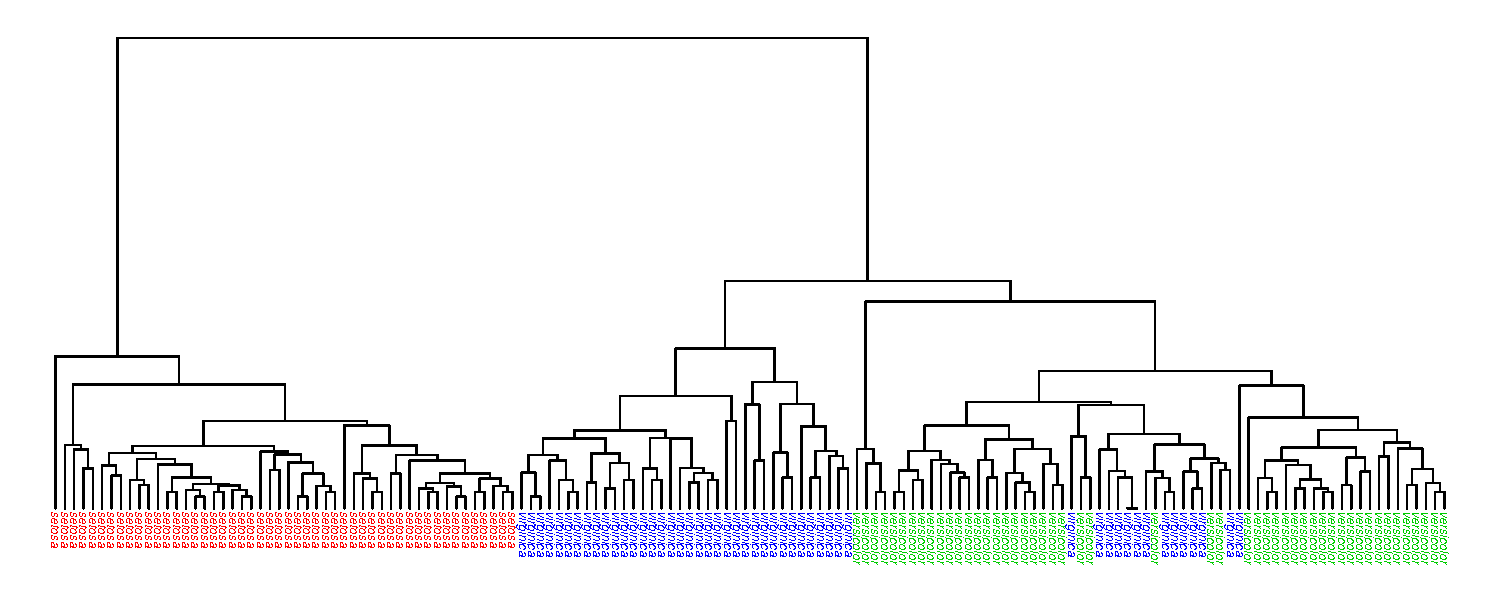
\includegraphics[width=6.5in]{pbdDEMO-include/pics/dist_iris}
\caption{Hierarchical clustering result of \code{iris}\ dataset.}
\label{fig:dist_iris}
\end{figure}


\section{Neighbor Joining}

In some sense, Figure~\ref{fig:dist_iris} is a rooted tree and the
``average'' method as well as UPGMA assumes a constant rate of evolution
(molecular clock hypothesis). However, these assumption may not be
appropriate to most sequence evolutionary topics where a gene tree should
be more suitable to interpret relation of sequences or species.
We introduce a popular approach in evolution biology and build a
evolutionary tree for {\it Pony 524} dataset\index{Data!Pony 524}.
We select JC69 evolutionary model~\citep{Jukes1969} as a probability measure
to compute for distance (evolution time) of 146 EIAV sequences and
use a neighbor joining tree~\citep{Saitou1987}\index{Algorithm!neighbor-joining}
to build an unrooted tree.

The purpose is to design a wrapper function, says \code{my.dist(x, y)},
that takes a pairs of sequences \code{x} and \code{y} as inputs, and
returns a user-defined distance of given data.
The utility function \code{comm.pairwise()}\index{Code!\code{comm.pairwise()}}
of \pkg{pbdMPI}~\citep{Chen2012pbdMPIpackage}
is more flexible than \code{comm.dist()}.
Through the options \code{pairid.gbd} and \code{FUN = my.dist}, the
function can evaluate \code{my.dist()} on the given dataset \code{X} in
row major blocks.
For {\it Pony 524}, the \code{X} is the DNA sequences and \code{my.dist()}
is a wrapper of \code{phyclust.edist}\index{Code!\code{phyclust.edist()}}.

The example in SPMD can be found in demo via
\begin{lstlisting}
### At the shell prompt, run the demo with 4 processors by
### (Use Rscript.exe for windows system)
mpiexec -np 4 Rscript -e "demo(dist_pony,'pbdDEMO',ask=F,echo=F)"
\end{lstlisting}
and it returns a neighbor-joining tree as Figure~\ref{fig:dist_pony}.

\begin{figure}[h!tb]
\centering
 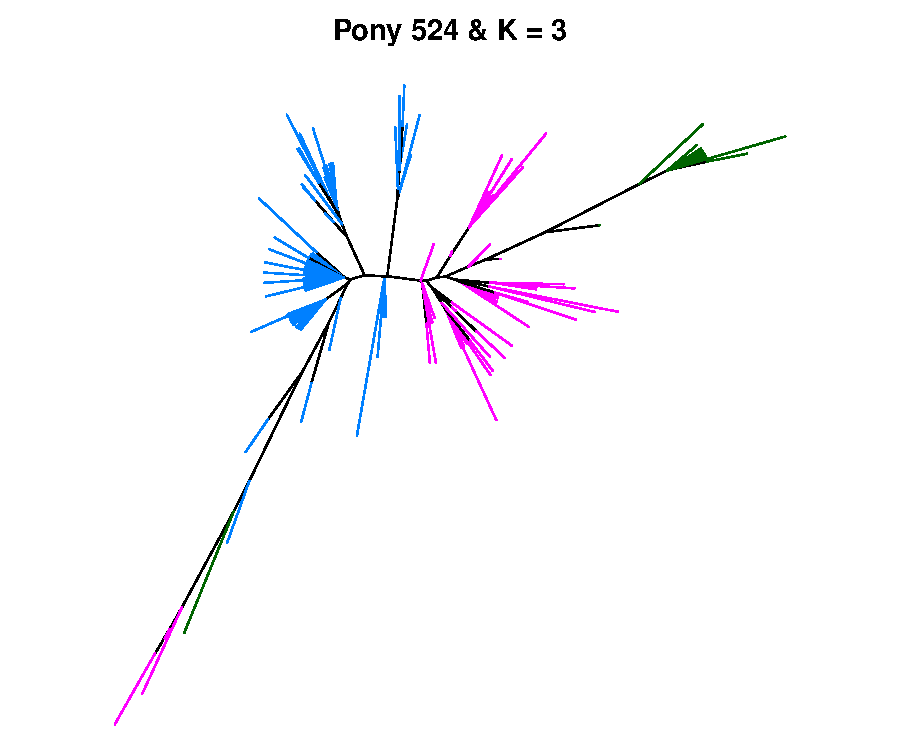
\includegraphics[width=4.5in]{pbdDEMO-include/pics/dist_pony}
\caption{Neighbor-joining tree of {\it Pony 524} dataset colored by three
         clusters.}
\label{fig:dist_pony}
\end{figure}


\section{Exercises}
\label{sec:pairwise_exercise}

\begin{enumerate}[label=\thechapter-\arabic*]

\item
What are potential limitations of distance approaches?

\item
Prove that clustering based on Euclidean distance is equivalent to that
clustering based on multivariate Normal distributions with identity variance
covariance matrices.

\item
Prove that the ``average'' method of \code{hclust()} is equivalent to the
UPGMA method.

\item
Given $n$ observations or taxa, analytically find total numbers of possible
rooted and unrooted trees, $(2n-5)!!$ and $(2n-3)!!$, respectively.

\item
As number of observations increases, the data and the distance matrix are
both distributed as the category (C4). State potential problems of
implementations and minimum costs of communications.

\item
Discuss the difficulties and problems of designing tree algorithms on a
distributed manner.

\end{enumerate}

